\documentclass[12pt,a4paper,oneside]{report}

\usepackage{amsthm}
\usepackage{amsmath}
\usepackage{tikz}
\usetikzlibrary{shapes,arrows,automata,trees, shadows,decorations.pathmorphing}
\begin{document}
\title{CS375 Week 6}
\author{Jason N Mansfield}
\maketitle
%1
\section{}

$$\mathbf{L =\{a^n b^{2n}\mid n \ge 1\} = \{abb, aabbbb, aaabbbbbb,...\}}$$



\begin{proof}
For any regular language L, there exists a number p such that for any string w in L of length at least p there are strings x,y,z such that
\begin{itemize}
\item $w =  xyz$
\item $\mid xy \mid \le  p$
\item $\mid y \mid \ge 1$
\item Then $x = a^n, y = a^n, z = b^{p+1}$
\item $xy^2z \ni L$
\item This is a contradiction so the shown language is nonregular.
\end{itemize}
\end{proof}

\begin{figure}
\begin{center}
\caption{Pumping Lemma Contradiction}
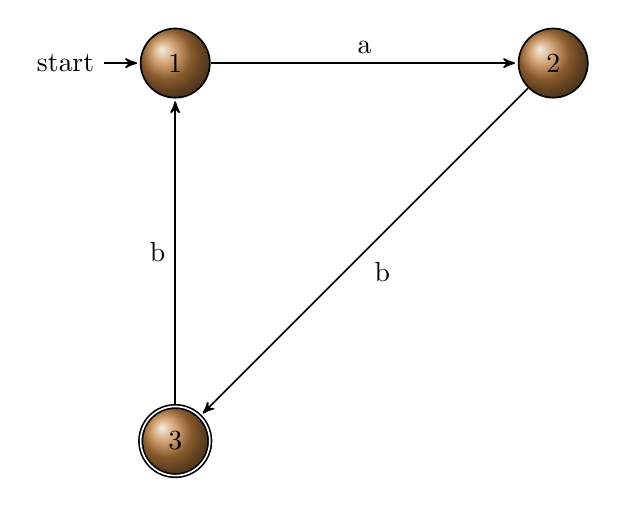
\begin{tikzpicture}[->,>=stealth',shorten >=1pt,auto,node distance=4.8cm, semithick]
\tikzstyle{every state}=[draw=black,text=black, ball color=brown]
\node[initial,state] (1) {1};
\node[state][right of=1](2){2};
\node[state, accepting][below of=1](3){3};
\path (1)edge node{a}(2)
          (2)edge node{b}(3)
          (3)edge node{b}(1);       
\end{tikzpicture} 
\end{center}
\end{figure}
%2
\section{}
\begin{enumerate}
\item Palindromes
\begin{proof}
For any regular language L, there exists a number p such that for any string w in L of length at least p there are strings x,y,z such that
\begin{enumerate}
\item If w = xyz.
\item And if x = a, y = b, z = a.
\item or if x = b, y = a, z = b.
\item Then $w = a^{90 + 1}ba^{90}$
\item and $w = b^{90 + 1}ab^{90}$
\item Therefore Palindromes are nonregular
\end{enumerate}
\end{proof}
\item Equal
\begin{proof}
For any regular language L, there exists a number p such that for any string w in L of length at least p there are strings x,y,z such that
\begin{enumerate}
\item  EQUAL = $\{\Lambda \quad ab \quad ba \quad aabb \quad abab \quad abba \quad baab \quad baba \quad bbaa \quad aaabbb...\}$
\item $\{a^nb^n\} = \mathbf{a^*b^*} \cap EQUAL$
\item If $a^*b^*$ is regular then so is the result of $\mathbf{a^*b^*} \cap EQUAL$
\item $w =  xyz$
\item $\mid xy \mid \le  p$
\item $\mid y \mid \ge 1$
\item Then $x = a^n, y = a^2, z = b^n$
\item So then xyyz would allow aaab which is not in this language.
\item Therefore this language is nonregular
\end{enumerate}
\end{proof}
\end{enumerate}
%3
\section{}
Prove that the below generates the language defined by the regular expression: $\mathbf{a^*bb}$
$$\mathbf {Prod 1 \quad S \to aS \mid bb}$$
\begin{equation}
\begin{split}
&S \Longrightarrow aS\\
&\Longrightarrow aaS\\
&\Longrightarrow aaaS\\
&\Longrightarrow aaaaS\\
&\Longrightarrow aaaaaS\\
&\Longrightarrow aaaaabb\\
\end{split}
\end{equation}
This derivation could continue infinitely until terminal bb is appended.
%4
\section{}
To generate aabbab using: $a(a +b)*$
\begin{equation}
\begin{split}
&\mathbf {Prod 1 \quad S \to aX}\\
&\mathbf{Prod 2 \quad X \to aX \mid bX \mid \Lambda}\\
&S \Longrightarrow aX \quad \text{(by Prod 1)}\\
&\Longrightarrow aaX \quad \text{(by Prod 2)}\\
&\Longrightarrow aabX \quad \text{(by Prod 2)}\\
&\Longrightarrow aabbX \quad \text{(by Prod 2)}\\
&\Longrightarrow aabbaX \quad \text{(by Prod 2)}\\
&\Longrightarrow aabbabX \quad \text{(by Prod 2)}\\
&\Longrightarrow aabbab\Lambda \quad \text{(by Prod 2)}\\
\end{split}
\end{equation}
%5
\section{}
To generate bbabaaa using: $(a + b)^*a(a + b)^*a(a + b)^*$
\begin{equation}
\begin{split}
&\mathbf {Prod 1 \quad S \to XaXaX}\\
&\mathbf {Prod 2 \quad X \to aX \mid bX \mid \Lambda}\\
&S \Longrightarrow XaXaX \quad \text{(by Prod 1)}\\
&\Longrightarrow XaXaaX \quad \text{(by Prod 2)}\\
&\Longrightarrow bXaXaaX \quad \text{(by Prod 2)}\\
&\Longrightarrow bXaXaa \quad \text{(by Prod 2)}\\
&\Longrightarrow bXabXaa \quad \text{(by Prod 2)}\\
&\Longrightarrow bXabaXaa \quad \text{(by Prod 2)}\\
&\Longrightarrow bbXabaXaa \quad \text{(by Prod 2)}\\
&\Longrightarrow bbabaXaa \quad \text{(by Prod 2)}\\
&\Longrightarrow bbabaaa \quad \text{(by Prod 2)}\\
\end{split}
\end{equation}
%6
\section{}
\begin{equation}
\begin{split}
&\mathbf {Prod 1 \quad S \to Xa}\\
&\mathbf {Prod 2 \quad X \to bbX \mid bbS \mid bb\mid\Lambda}\\
\end{split}
\end{equation}
\clearpage
%7
\section{}
%sub1
\subsection{}
This CFG cannot match aaaa, abaa, or bbaa. The only string of length 4 is aabb:
\begin{equation}
\begin{split}
&\mathbf {Prod 1 \quad S \to aSb \mid ab}\\
\end{split}
\end{equation}
\begin{center}
\begin{tikzpicture}[level 1/.style={sibling distance=6em},
                   level 2/.style={sibling distance=1em}, level distance=2cm,draw=green]]
\node {S}
child {node {aSb} child {node {S} child {node {a}} child {node {S}child {node{ab}}} child {node{b}}}}
child {node {ab}}
;
\end{tikzpicture} 
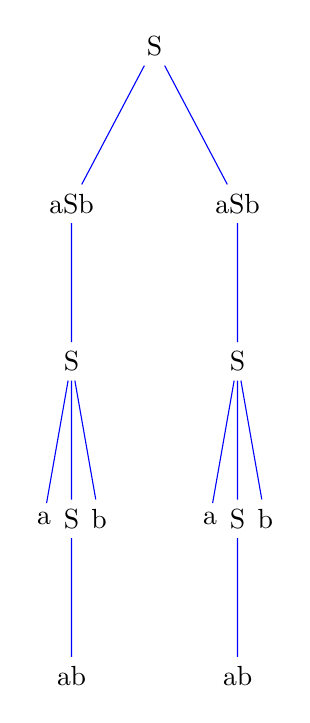
\begin{tikzpicture}[level 1/.style={sibling distance=6em},
                   level 2/.style={sibling distance=1em}, level distance=2cm,draw=blue]]
\node {S}
child {node {aSb} child {node {S} child {node {a}} child {node {S}child {node{ab}}} child {node{b}}}}
child {node {aSb} child {node {S} child {node {a}} child {node {S}child {node{ab}}} child {node{b}}}}
;
\end{tikzpicture} 
\begin{tikzpicture}[level 1/.style={sibling distance=6em},
                   level 2/.style={sibling distance=1em}, level distance=2cm,draw=red]]
\node {S}
child {node {ab}}
child {node {aSb} child {node {S} child {node {a}} child {node {S}child {node{ab}}} child {node{b}}}}
;
\end{tikzpicture} 
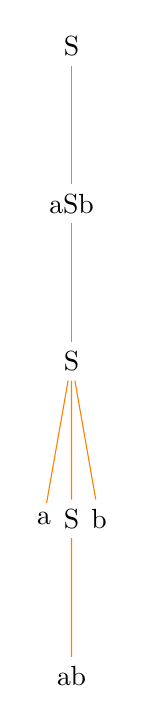
\begin{tikzpicture}[level 1/.style={sibling distance=6em},
                   level 2/.style={sibling distance=1em}, level distance=2cm,draw=orange]]
\node {S}
child {node {aSb} child {node {S} child {node {a}} child {node {S}child {node{ab}}} child {node{b}}}}
;
\end{tikzpicture} 
\end{center}
\clearpage
%sub2
\subsection{}
For strings aaaa, abaa, or bbaa. This CFG can create the string aaaa, bbaa:
\begin{equation}
\begin{split}
&\mathbf {Prod 1 \quad S \to aS \mid bS \mid a}\\
\end{split}
\end{equation}
\begin{center}
\begin{tikzpicture}[level 1/.style={sibling distance=6em},
                   level 2/.style={sibling distance=1em}, level distance=2cm,draw=red]]
\node {S}
child {node {aS} child{node{S} child {node {a}}child {node {a}}}}
child {node {a}}
child {node {a}}
;
\end{tikzpicture} 
\begin{tikzpicture}[level 1/.style={sibling distance=6em},
                   level 2/.style={sibling distance=1em}, level distance=2cm,draw=blue]]
\node {S}
child {node {bS}child{node{S} child {node {b}}child {node {S} child {node {bS} child {node{S} child{node {b}} child{node{S} child{node{a}}}}}}}}
child {node {a}}
;
\end{tikzpicture} 
\begin{tikzpicture}[level 1/.style={sibling distance=6em},
                   level 2/.style={sibling distance=1em}, level distance=2cm,draw=orange]]
\node {S}
child {node {bS}child{node{S} child {node {a}}child {node {S} child {node {bS} child {node{S} child{node {b}} child{node{S} child{node{a}}}}}}}}
child {node {a}}
;
\end{tikzpicture} 
\end{center}
\clearpage
%sub3
\subsection{}
For strings aaaa, abaa, or bbaa. This CFG can create the string aaaa, abaa:
\begin{equation}
\begin{split}
&\mathbf {Prod 1 \quad S \to aS \mid aSb \mid X}\\
&\mathbf {Prod 2 \quad X \to aXa \mid a}\\
\end{split}
\end{equation}
\begin{center}
\begin{tikzpicture}[level 1/.style={sibling distance=14em},
                   level 2/.style={sibling distance=1.5em}, level distance=2cm,draw=red]]
\node {S}
child {node {a}}
child{node{S} child{node{X} child{node{a}}child{node{X}child{node{a}}}child{node{a}}}}
;
\end{tikzpicture} 
\begin{tikzpicture}[level 1/.style={sibling distance=14em},
                   level 2/.style={sibling distance=1.5em}, level distance=2cm,draw=blue]]
\node {S}
child {node {S} child{node{a}} child{node{b}}}
child {node {X} child{node{a}} child{node{a}}}

;
\end{tikzpicture} 
\end{center}
\clearpage
%sub4
\subsection{}
For strings aaaa, abaa, or bbaa. This CFG can create the string aaaa, abaa:
\begin{equation}
\begin{split}
&\mathbf {Prod 1 \quad S \to aAS \mid a}\\
&\mathbf {Prod 2 \quad A \to SbA \mid SS \mid ba}\\
\end{split}
\end{equation}
\begin{center}
\begin{tikzpicture}[level 1/.style={sibling distance=6em},
                   level 2/.style={sibling distance=1em}, level distance=2cm, draw=green!40!orange!90!]]
\node {S}
child {node {a}}
child {node {A} child{node {S}child {node {a}}} child{node {S}child {node {a}}}}
child {node {S}child {node {a}}}
;
\end{tikzpicture} 
\begin{tikzpicture}[level 1/.style={sibling distance=6em},
                   level 2/.style={sibling distance=1em}, level distance=2cm, draw=blue!40!orange!90!]]
\node {S}
child {node {a}}
child {node {A} child{node{ba}}}
child {node {S} child{node{a}}}
;
\end{tikzpicture} 
\end{center}
\clearpage
%sub5
\subsection{}
For strings aaaa, abaa, or bbaa. This CFG can create the string bbaa:
\begin{center}
\begin{equation}
\begin{split}
&\mathbf {Prod 1 \quad S \to aB \mid bA}\\
&\mathbf {Prod 2 \quad A \to a \mid aS \mid bAA}\\
&\mathbf{Prod 3 \quad B \to b \mid bS \mid aBB}\\
\end{split}
\end{equation}
\begin{tikzpicture}[level 1/.style={sibling distance=9em},
                   level 2/.style={sibling distance=1em}, level distance=3cm,draw=red!35!orange!90!]]
\node {S}
child {node {b}}
child {node {A} child{node{b}} child{node{A} child{node{a}}}child{node{A} child{node{a}}}}

;
\end{tikzpicture} 
\end{center}
\clearpage
%8
\section{}

\subsection{}
Ambiguous CFG with the string: babababab
\begin{equation}
\mathbf {Prod 1  \quad  S \to  SaSaS \mid b}
\end{equation}
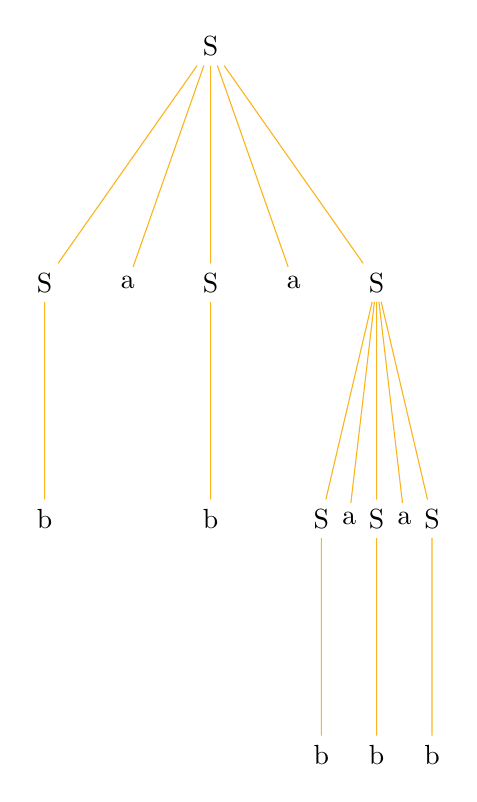
\begin{tikzpicture}[level 1/.style={sibling distance=3em},
                   level 2/.style={sibling distance=1em}, level distance=3cm,draw=yellow!35!orange!90!]]
\node {S}
child {node {S} child{node{b}}}
child {node {a}}
child {node {S} child{node{b}}}
child {node {a}}
child {node {S} child{node{S} child{node{b}}} child{node{a}} child{node{S} child{node{b}}} child{node{a}} child{node{S} child{node{b}}}}

;
\end{tikzpicture} 
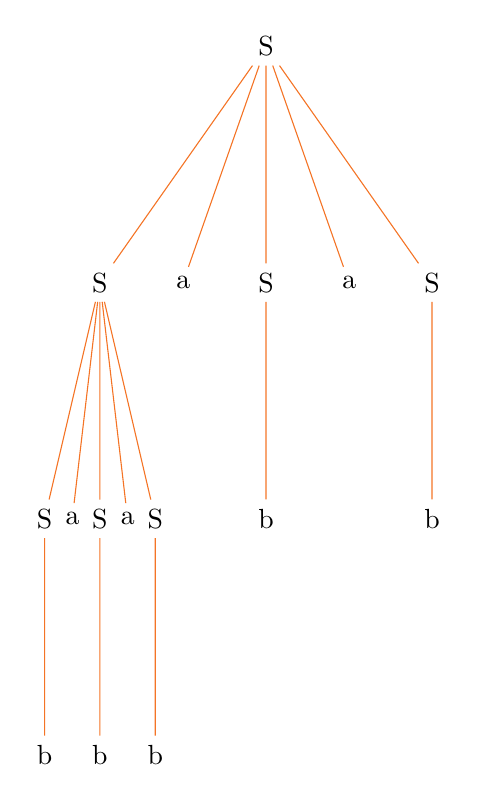
\begin{tikzpicture}[level 1/.style={sibling distance=3em},
                   level 2/.style={sibling distance=1em}, level distance=3cm,draw=yellow!35!red!90!]]
\node {S}
child {node {S} child{node{S} child{node{b}}} child{node{a}} child{node{S} child{node{b}}} child{node{a}} child{node{S} child{node{b}}}}
child {node {a}}
child {node {S} child{node{b}}}
child {node {a}}
child {node {S} child{node{b}}}
;
\end{tikzpicture} 
\clearpage
\subsection{}
\begin{center}
Ambiguous CFG with the string: aaaaaa
\begin{equation}
\mathbf {Prod 1 \quad  S \to aaS \mid aaaS \mid a}
\end{equation}
\begin{tikzpicture}[level 1/.style={sibling distance=4em},
                   level 2/.style={sibling distance=1em}, level distance=3cm,draw=red!35!blue!90!]]
\node {S}
child {node {a}}
child {node {a}}
child {node {S} child{node{a}}child{node{a}} child{node{a}} child{node{S} child{node{a}}}}
;
\end{tikzpicture} 
\begin{tikzpicture}[level 1/.style={sibling distance=4em},
                   level 2/.style={sibling distance=1em}, level distance=3cm,draw=red!35!brown!90!]]
\node {S}
child {node {a}}
child {node {a}}
child{node {a}}
child {node {S} child{node{a}} child{node{a}} child{node{S} child{node{a}}}}
;
\end{tikzpicture} 
\end{center}
\clearpage
\subsection{}
Ambiguous CFG with the string: aaaba
\begin{equation}
\begin{split}
&\mathbf {Prod 1  \quad S \to AA }\\
&\mathbf {Prod 2 \quad  A \to  AAA \mid a \mid bA \mid Ab}
\end{split}
\end{equation}
\begin{center}
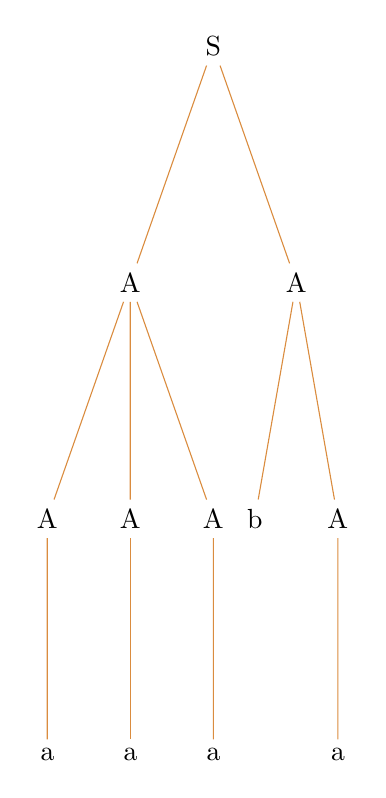
\begin{tikzpicture}[level 1/.style={sibling distance=6em},
                   level 2/.style={sibling distance=3em}, level distance=3cm,draw=orange!35!brown!90!]]
\node {S}
child {node {A} child{node{A} child {node{a}}} child{node{A}child {node{a}}} child{node{A}child {node{a}}}}
child {node {A} child{node{b}} child {node{A}child {node{a}}}}

;
\end{tikzpicture} 
\begin{tikzpicture}[level 1/.style={sibling distance=6em},
                   level 2/.style={sibling distance=3em}, level distance=3cm,draw=red!55!brown!90!]]
\node {S}
child {node {A} child{node{a}}}
child {node {A} child{node{A} child{node{a}}} child{node{A} child{node{A} child{node{a}}} child{node{b}} }child{node{A} child{node{a}}}}

;
\end{tikzpicture} 
\end{center}
\clearpage
%9
\section{}
%sub 9.1
\subsection{}

\begin{equation}
\begin{split}
&\mathbf {Prod 1 \quad S \to  XaX }\\
&\mathbf {Prod 2 \quad X \to  aX \mid bX \mid \Lambda }
\end{split}
\end{equation}
\subsubsection{Ambiguous}
\begin{equation}
\begin{split}
&S \Longrightarrow XaX\\
&X \Longrightarrow aXaX\\
&\quad \Longrightarrow a\Lambda aX\\
&\quad \Longrightarrow aaX\\
&\quad \Longrightarrow aa\Lambda\\
&\quad \Longrightarrow aa\\
\end{split}
\end{equation}
Second Example
\begin{equation}
\begin{split}
&S \Longrightarrow XaX\\
&X \Longrightarrow \Lambda aX\\
&\quad \Longrightarrow aaX\\
&\quad \Longrightarrow aa\Lambda\\
&\quad \Longrightarrow aa\\
\end{split}
\end{equation}
\begin{center}
\begin{tikzpicture}[level 1/.style={sibling distance=4em},
                   level 2/.style={sibling distance=2em}, level distance=2cm,draw=yellow!35!brown!90!]]
\node {S}
child{node{X} child{node{a}} child{node{X} child{node{$\Lambda$}}}}
child{node{a}}
child{node{X} child{node{$\Lambda$}}}

;
\end{tikzpicture} 
\begin{tikzpicture}[level 1/.style={sibling distance=4em},
                   level 2/.style={sibling distance=2em}, level distance=2cm,draw=yellow!35!green!90!]]
\node {S}
child{node{X} child{node{$\Lambda$}}}
child{node{a}}
child{node{X} child{node{a}} child{node{X} child{node{$\Lambda$}}}}
;
\end{tikzpicture} 
\end{center}
\subsubsection{Non-Ambiguous}
\begin{equation}
\begin{split}
&S \Longrightarrow XaX\\
&X \Longrightarrow aXaX\\
&\quad \Longrightarrow aaXaX\\
&\quad \Longrightarrow aaaXaX\\
&\quad \Longrightarrow aaa \Lambda aX\\
&\quad \Longrightarrow aaaaaX\\
&\quad \Longrightarrow aaaaaaX\\
&\quad \Longrightarrow aaaaaaaX\\
&\quad \Longrightarrow aaaaaaa \Lambda \\
&\quad \Longrightarrow aaaaaaa
\end{split}
\end{equation}
\begin{center}
\begin{tikzpicture}[level 1/.style={sibling distance=4em},
                   level 2/.style={sibling distance=2em}, level distance=2cm,draw=yellow!15!blue!90!]]
\node {S}
child{node{X} child{node{a}} child{node{X} child{node{a}} child{node{X} child{node{a}} child{node{X} child{node{$\Lambda$}}} }}}
child{node{a}}
child{node{X} child{node{a}} child{node{X} child{node{a}} child{node{X} child{node{a}} child{node{X} child{node{$\Lambda$}}}}}}
;
\end{tikzpicture} 
\end{center}
Second Example
\begin{equation}
\begin{split}
&S \Longrightarrow XaX\\
&X \Longrightarrow bXaX\\
&\quad \Longrightarrow bbXaX\\
&\quad \Longrightarrow bbbXaX\\
&\quad \Longrightarrow bbb \Lambda aX\\
&\quad \Longrightarrow bbbbbX\\
&\quad \Longrightarrow bbbbbbX\\
&\quad \Longrightarrow bbbbbbbX\\
&\quad \Longrightarrow bbbbbbb \Lambda \\
&\quad \Longrightarrow bbbbbbb
\end{split}
\end{equation}


\begin{tikzpicture}[level 1/.style={sibling distance=4em},
                   level 2/.style={sibling distance=2em}, level distance=2cm,draw=red!75!blue!70!]]
\node {S}
child{node{X} child{node{b}} child{node{X} child{node{b}} child{node{X} child{node{b}} child{node{X} child{node{$\Lambda$}}}}}}
child{node{a}}
child{node{X} child{node{b}} child{node{X} child{node{b}} child{node{X} child{node{b}} child{node{X} child{node{$\Lambda$}}}}}}
;
\end{tikzpicture} 
\clearpage
% sub 9.2
\subsection{}
\subsubsection{Ambiguous}
\begin{equation}
\begin{split}
&\mathbf {Prod 1 \quad  S \to  aSX\mid \Lambda}\\
&\mathbf {Prod 2 \quad  X\to  aX \mid a}
\end{split}
\end{equation}
\begin{equation}
\begin{split}
&S \Longrightarrow aSX\\
&\quad \Longrightarrow a \Lambda X\\
& \quad \Longrightarrow aX\\
&\quad \Longrightarrow aaSX\\
&\quad \Longrightarrow aa \Lambda X\\
&\quad \Longrightarrow aaa\\
\end{split}
\end{equation}
Second Example
\begin{equation}
\begin{split}
&S \Longrightarrow aSX\\
&\quad \Longrightarrow aXX\\
& \quad \Longrightarrow aaX\\
&\quad \Longrightarrow aaaSX\\
&\quad \Longrightarrow aaa \Lambda X\\
&\quad \Longrightarrow aaa \Lambda \\
\end{split}
\end{equation}
\begin{center}
\begin{tikzpicture}[level 1/.style={sibling distance=4em},
                   level 2/.style={sibling distance=2em}, level distance=2cm,draw=yellow!75!blue!70!]]
\node {S}
child{node{a}}
child{node{S}child{node{$\Lambda$}}}
child{node{X} child{node{a}} child{node{S} child{node{$\Lambda$}}} child{node{X} child{node{a}}}}
;
\end{tikzpicture} 
\begin{tikzpicture}[level 1/.style={sibling distance=4em},
                   level 2/.style={sibling distance=2em}, level distance=2cm,draw=orange!75!blue!70!]]
\node {S}
child{node{a}}
child{node{S}child{node{X} child{node{a}}}}
child{node{X} child{node{a}} child{node{S} child{node{$\Lambda$}}} child{node{X} child{node{$\Lambda$}}}}
;
\end{tikzpicture} 
\end{center}
\subsubsection{Non-Ambiguous}
\begin{equation}
\begin{split}
&S \Longrightarrow aSX\\
&\quad \Longrightarrow aaSXX\\
&\quad \Longrightarrow aaaSXXa\\
&\quad \Longrightarrow aaa \Lambda Xaa\\
&\quad \Longrightarrow aaaaaa\\
\end{split}
\end{equation}
\begin{tikzpicture}[level 1/.style={sibling distance=7em},
                              level 2/.style={sibling distance=6em},
                              level 3/.style={sibling distance=5em},
                              level distance=2cm,draw=orange!75!yellow!70!]]
                   
\node {S}
child{node{a}}
child{node{S}child{node{a}}
child{node{S}child{node{a}}
child{node{S} child{node{$\Lambda$}}}
child{node{X}child{node{a}}}}
child{node{X}child{node{a}}}}
child{node{X}child{node{a}}}

;
\end{tikzpicture} 
\clearpage
%sub 9.3
\subsection{}
\begin{equation}
\mathbf {Prod 1 \quad  S\to  aS \mid bS \mid aaS \mid \Lambda}
\end{equation}
\subsubsection{Ambiguous}

\begin{equation}
\begin{split}
&S \Longrightarrow aS\\
&\quad \Longrightarrow aaS\\
&\quad \Longrightarrow aaaS\\
&\quad \Longrightarrow aaa \Lambda\\
&\quad \Longrightarrow aaa 
\end{split}
\end{equation}
Second Example
\begin{equation}
\begin{split}
&S \Longrightarrow aaS\\
&\quad \Longrightarrow aaaS\\
&\quad \Longrightarrow aaa \Lambda\\
&\quad \Longrightarrow aaa 
\end{split}
\end{equation}

\begin{center}
\begin{tikzpicture}[level 1/.style={sibling distance=4em},
                   level 2/.style={sibling distance=2em}, level distance=2cm,draw=orange!75!blue!70!]]
\node {S}
child{node{a}}
child{node{S} child{node{a}} child{node{a}} child{node{S} child{node{$\Lambda$}}}}
;
\end{tikzpicture} 
\begin{tikzpicture}[level 1/.style={sibling distance=4em},
                   level 2/.style={sibling distance=2em}, level distance=2cm,draw=red!75!purple!70!]]
\node {S}
child{node{a}}
child{node{a}}
child{node{S} child{node{a}} child{node{S} child{node{$\Lambda$}}}}
;
\end{tikzpicture} 
\end{center}
\clearpage
\subsubsection{Non-Ambiguous}
\begin{equation}
\begin{split}
&S \Longrightarrow bS\\
&\quad \Longrightarrow bbS\\
&\quad \Longrightarrow bbbS\\
&\quad \Longrightarrow bbb \Lambda\\ 
&\quad \Longrightarrow bbb 
\end{split}
\end{equation}
\begin{center}
\begin{tikzpicture}[level 1/.style={sibling distance=4em},
                   level 2/.style={sibling distance=4em}, level distance=2cm,draw=orange!75!green!70!]]
\node {S}
child{node{b}}
child{node{S}child{node{b}}
child{node{S}child{node{b}}
child{node{S}child{node{$\Lambda$}}}}}

;
\end{tikzpicture} 
\end{center}
\clearpage
%10
\section{}
\subsection{}
\begin{equation}
\mathbf {Prod 1 \quad  S \to aS \mid bS \mid a}
\end{equation}
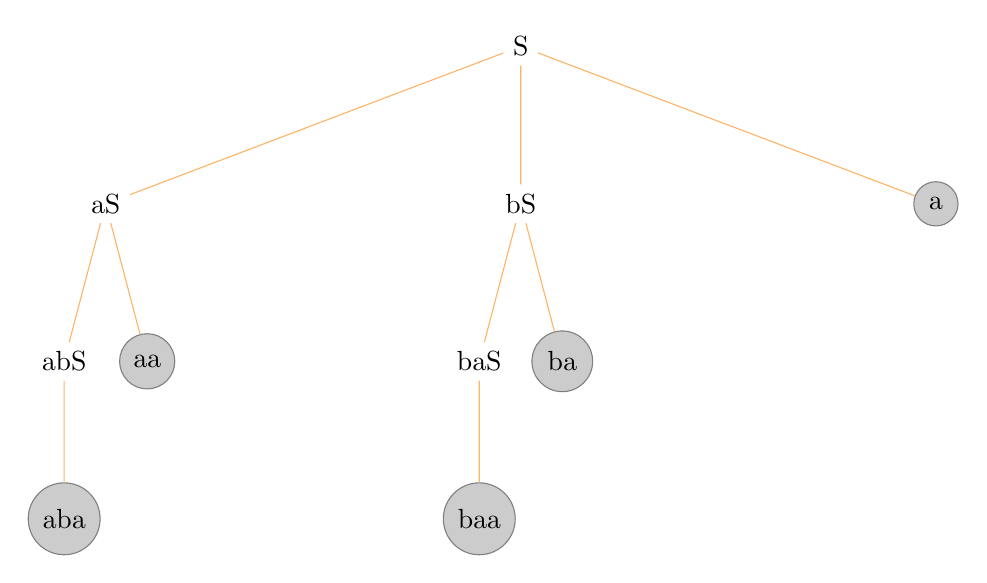
\begin{tikzpicture}[level 1/.style={sibling distance=15em},
                   level 2/.style={sibling distance=3em}, level distance=2cm,draw=orange!85!white!70!]]
\node {S}
child{node{aS} child{node{abS} 
child{node[shape=circle,draw=black!50,fill=black!20]{aba}} }
child{node[shape=circle,draw=black!50,fill=black!20]{aa}}}
child{node{bS} child{node{baS} 
child{node[shape=circle,draw=black!50,fill=black!20]{baa}}} 
child{node[shape=circle,draw=black!50,fill=black!20]{ba}}}
child{node[shape=circle,draw=black!50,fill=black!20]{a}}

;
\end{tikzpicture} 
\subsection{}
\begin{equation}
\begin{split}
&\mathbf {Prod 1 \quad  S \to aSb \mid bX}\\
&\mathbf{Prod 2 \quad X \to bX \mid b}
\end{split}
\end{equation}
\begin{center}
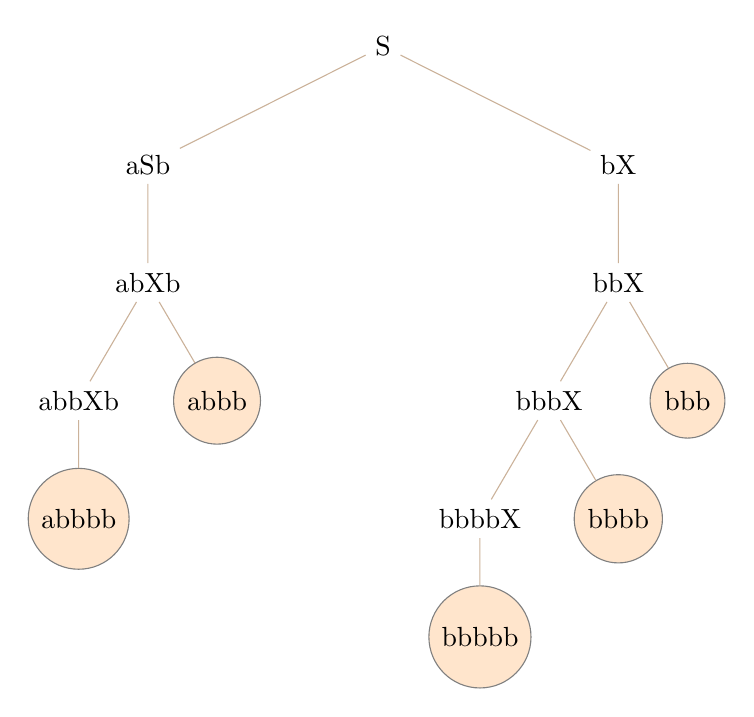
\begin{tikzpicture}[level 1/.style={sibling distance=17em},
                   level 2/.style={sibling distance=5em}, level distance=1.5cm,draw=gray!35!brown!60!]]
\node {S}
child{node{aSb} child{node{abXb} child{node{abbXb}child{node[shape=circle,draw=black!50,fill=orange!20]{abbbb}}} 
child{node[shape=circle,draw=black!50,fill=orange!20]{abbb}}}}
child{node{bX} child{node {bbX} child{node{bbbX}child{node{bbbbX} 
child{node[shape=circle,draw=black!50,fill=orange!20]{bbbbb}}} 
child{node[shape=circle,draw=black!50,fill=orange!20]{bbbb}}}
child{node[shape=circle,draw=black!50,fill=orange!20]{bbb}}}}


;
\end{tikzpicture} 
\end{center}
\clearpage
%11
\section{}
The CFG's generated by the Regular Languages over the alphabet $\Sigma = \{a b \}$:
\subsection{}
The language defined by $(aaa + b)^*$:
\subsection{}
The language defined by $(a + b)^*(bbb + aaa)(a + b)^*$:
\subsection{}
All the strings that end in b and have an even number of b's in total:
\subsection{}
The set of all strings of odd length:
\subsection{}
All strings with exactly one a or exactly one b:
\subsection{}
All strings with an odd number of a's or and even number of b's:
\end{document}